\documentclass[a4paper, 12pt]{article}

% -- Language --
\usepackage[spanish]{babel}
\usepackage[utf8]{inputenc}

% ----- Fonts -----
% -- Color --
\usepackage{xcolor}
%\definecolor{azul}{RGB}{00,33,99}
\definecolor{azul}{RGB}{35,72,180}

% -- Page Margin --
\usepackage[margin=1in]{geometry}

% -- Espaciados --
\newcommand{\Pspace}{0.5cm}
\newcommand{\Aspace}{0.2cm}

% -- Imagenes --
\usepackage{graphicx}
\usepackage{float}

% -- Matemáticas --
\usepackage{amsmath, amssymb}

% -- Gráficas --
\usepackage{pgfplots}
\pgfplotsset{compat=1.18}

% -- Código --
\usepackage{listings}
\lstset{
    language=C++,                   % Lenguaje del código
    basicstyle=\ttfamily\small,     % Fuente del código
    keywordstyle=\color{blue},      % Color de palabras clave
    commentstyle=\color{gray},      % Color de comentarios
    stringstyle=\color{red},        % Color de cadenas
    numbers=left,                   % Números de línea a la izquierda
    numberstyle=\tiny\color{gray},
    breaklines=true,                % Permitir saltos de línea
    frame=single                    % Marco alrededor del código
}


\title
{
    Probabilidad 2025-1 \\
    Tareas Parcial 3
    }

    \begin{document}

    \maketitle

    \begin{center}
        \begin{tabular}{r|l}
            \textbf{Expediente} & \textbf{Nombre} \\ \hline
            219208106 & Bórquez Guerrero Angel Fernando \\
            223203899 & Tostado Cortes Dante Alejandro \\
        \end{tabular}
    \end{center}

    \rule{\linewidth}{0.3mm}



    % ---------- Tarea 9 ----------
    \vspace{0.3cm}

    \begin{center}
        { \LARGE Tarea 9}
    \end{center}

    \begin{enumerate}
        % - Problema 1
        \item Comprobar si la siguiente función es de probabilidad \par
        \[
            f(x) =
            \begin{cases}
                \frac{1 / 2}{\sqrt{x}} & 0 < x < 1 \\
                0 & \text{Otro caso}
            \end{cases}
        \]
            % Respuesta:
            \vspace{\Aspace}
            { \color{azul} 
                \[  \int_{0}^{1}\frac{\frac{1}{2}}{\sqrt{x}}dx 
                    = \frac{1}{2} \int_{0}^{1}x^{-\frac{1}{2}}dx
                    = \frac{1}{2} \left[ \frac{\sqrt{x}}{\frac{1}{2}} \Big|_{0}^{1} \right]
                    = \sqrt{x} \Big|_{0}^{1}
                    = \sqrt{1} - \sqrt{0} = 1
                \]
            }
        
        \newpage
        % - Problema 2
        \vspace{\Pspace}
        \item Encontrar la función de distribución con la función de probabilidad
        \[
            f(x) =
            \begin{cases}
                2x & 0 \leq x \leq 1 \\
                0 & \text{Otro caso}
            \end{cases}
        \]       
        Grafica ambas funciones
            % Respuestas:
            \vspace{\Aspace} \par
            { \color{azul} 
                a) Función de probabilidad: \par
                \begin{figure}[H]
                    \centering
                    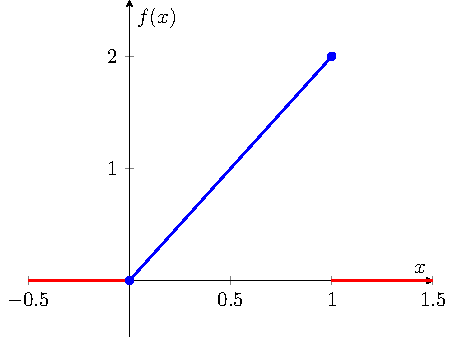
\includegraphics[width=0.5\textwidth]{Assets/Pdf/T9P2IA.pdf}
                \end{figure}

                b) Función de distribución:
                \[
                    F(x) = \int_{-\infty}^{x} 2u du
                    = 2 \int_{-\infty}^{x} u du =
                    \begin{cases}
                        0 & x < 0 \\
                        x^{2} & 0 \leq x \leq 1 \\
                        1 & x > 1                       
                    \end{cases}
                \]
                \begin{figure}[H]
                    \centering
                    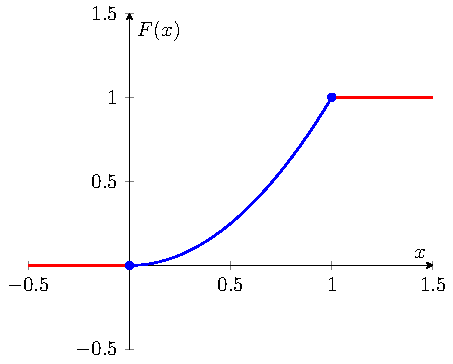
\includegraphics[width=0.5\textwidth]{Assets/Pdf/T9P2IB.pdf}
                \end{figure}
            }

        \newpage
        % - Problema 3
        \item Sea la función de distribución
        \[
            F(x) =
            \begin{cases}
                0 & x < 0 \\
                x & 0 \leq x \leq 1 \\
                1 & x > 1
            \end{cases}
        \]
        Determinar si se trata de la función de distribución de una variable aleatoria discreta o continua. Encontrar además la correspondiente función de probabilidad o densidad y graficarlas.
            % Respuestas:
            \vspace{\Aspace} \par
            { \color{azul} 
                Se trata de una variable continua. \par
                \vspace{\Aspace}
                a) Función de distribución:
                \begin{figure}[H]
                    \centering
                    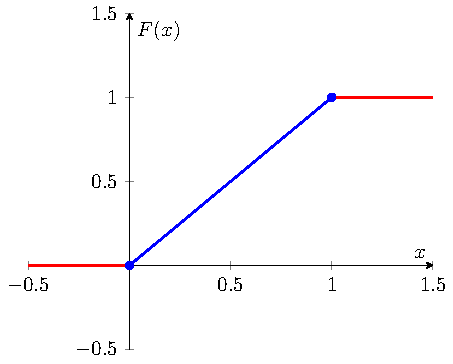
\includegraphics[width=0.5\textwidth]{Assets/Pdf/T9P3IA.pdf}
                \end{figure}

                b) Función de densidad:
                \[
                    \frac{d}{dx}F(x) = f(x) =
                    \begin{cases}
                        1   &   0 \leq x \leq 1     \\
                        0   &   \text{Otro caso}    \\
                    \end{cases}
                \]
                \begin{figure}[H]
                    \centering
                    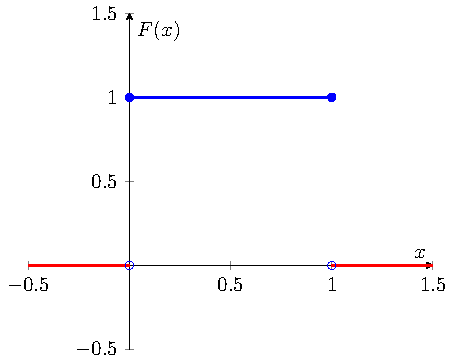
\includegraphics[width=0.5\textwidth]{Assets/Pdf/T9P3IB.pdf}
                \end{figure}
            }
    \end{enumerate}



    \newpage
    % ---------- Tarea 10 ----------
    \vspace{0.3cm}

    \begin{center}
        { \LARGE Tarea 10}
    \end{center}

    \begin{enumerate}
        % - Problema 1
        \item Encontrar el valor esperado y la desviación estándar de la función de densidad \par
        \[
            f(x) =
            \begin{cases}
                e^{-x} & x > 0 \\
                0 & \text{Otro caso}
            \end{cases}
        \]
            % Respuestas:
            \vspace{\Aspace}
            { \color{azul} 
                \begin{flushleft}
pwd | xclip -selection clipboard
                    a) Valor esperado:
                \end{flushleft}
                \[
                    E[X] 
                    = \int_{0}^{\infty} xe^{-x}dx
                    = -xe^{-x} + \int_{0}^{\infty} e^{-x}dx
                    = -xe^{-x}-e^{-x} \Big|_{0}^{\infty}
                    = -\frac{x + 1}{e^{x}} \Big|_{0}^{\infty}
                    = 1
                \]

                \begin{flushleft}
                    b) Varianza:
                \end{flushleft}
                \[
                    \text{Var}[X]
                    = \int_{0}^{\infty} x^{2}e^{-x}dx - \int_{0}^{\infty}(x - 1)^{2}e^{-x}dx
                    = 2 - 1
                    = 1
                \]
            }

        % - Problema 2
        \vspace{\Pspace}
        \item Encontrar la función de densidad y distribución con $U \sim U(0, 4)$. Graficas ambas funciones y encontrar el valor esperado y la desviación estándar.
            % Respuestas:
            \vspace{\Aspace} \par
            { \color{azul} 
                a) Función de densidad:
                \[
                    f(x) = 
                    \begin{cases}
                        \frac{1}{4} &   0 < x < 4 \\
                        0           &   \text{Otro caso}
                    \end{cases}
                \]
                \begin{figure}[H]
                    \centering
                    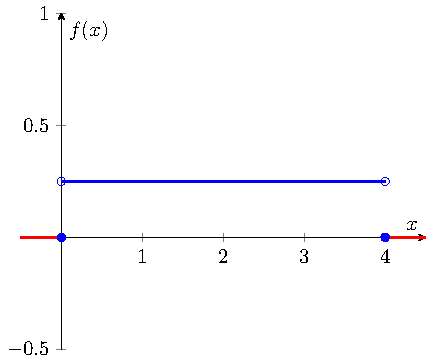
\includegraphics[width=0.5\textwidth]{Assets/Pdf/T10P2IA.pdf}
                \end{figure}

                \newpage
                b) Función de distribución:
                \[
                    F(x)
                    = \int_{0}^{x} \frac{1}{4}du
                    = \frac{1}{4} \int_{0}^{x}du
                    = \frac{u}{4} \Big|_{0}^{x}
                    = \frac{u}{4} =
                    \begin{cases}
                        0           &   x \leq 0 \\
                        \frac{x}{4} &   0 < x < 4 \\
                        1           &   x \geq 4
                    \end{cases}
                \]
                \begin{figure}[H]
                    \centering
                    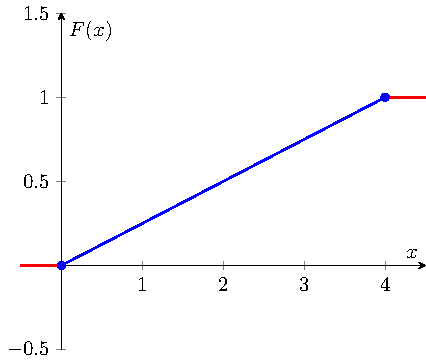
\includegraphics[width=0.5\textwidth]{Assets/Pdf/T10P2IB.pdf}
                \end{figure}

                c) Valor esperado:
                \[
                    E[X] = \frac{1}{4} \int_{0}^{4}xdx = \frac{x^{2}}{8}\Big|_{0}^{4} = 2
                \]

                d) Varianza:
                \[
                    Var[X] = E[X^{2}] - (E[X])^{2} 
                    = \frac{1}{4} \int_{0}^{4} x^{2}dx - 2^{2} 
                    = \frac{16}{3} - 4 
                    = \frac{4}{3}
                \]

                e) Deviación estándar:
                \[
                    \sigma = \sqrt{\frac{4}{3}}
                \]
            }

        \newpage
        % - Problema 3
        \item Sea $X$ una variable aleatoria con distribución uniforme entre $-1$ y $1$. Demuestre lo siguiente
        \[
            E[X^{n}] =
            \begin{cases}
                0 & \text{si $n$ es impar}  \\
                \frac{1}{n + 1} & \text{si $n$ es par} \\
            \end{cases}
        \]
            % Respuesta:
            \vspace{\Aspace} \par
            { \color{azul} 
                Función de densidad:
                \[
                    f(x) =
                    \begin{cases}
                        \frac{1}{2} &   -1 < x < 1 \\
                        0           &   \text{Otro caso}
                    \end{cases}
                \]

                Valor esperado de $X^{n}$
                \[
                    \frac{1}{2} \int_{-1}^{1} x^{n}dx
                    = \frac{x^{n + 1}}{2(n + 1)} \Big|_{-1}^{1}
                    = \frac{1^{n + 1}}{2(n + 1)} - \frac{(-1)^{n + 1}}{2(n + 1)}
                    = \frac{1 - (-1)^{n}(-1)}{2(n + 1)}
                    = \frac{1 + (-1)^{n}}{2(n + 1)}
                \]

                Queremos comprobar que cuando $n$ es impar la función vale 0 y cuando es par vale $\frac{1}{n + 1}$, para esto vamos a reescribir a $n$ como $2k$ para valores pares, como $2k + 1$ para valores impares y evaluamos por partes. \par
                - Cuando $n$ es par: \par
                • Reemplazamos $n$ por $2k$ en la función obtenida para el valor esperado de $X^{n}$.
                \[ \frac{1 + (-1)^{2k}}{2(2k + 1)} \]

                • Desarrollamos la funcíon.
                \[
                    \frac{1 + ((-1)^{2})^{k}}{2(2k + 1)}
                    = \frac{1 + (1)^{k}}{2(2k + 1)}
                    = \frac{1 + 1}{2(2k + 1)}
                    = \frac{2}{2(2k + 1)}
                    = \frac{1}{2k + 1}
                \]

                • Reemplazamos $2k$ por $n$.
                \[
                    \frac{1}{n + 1}
                \]
                
                \vspace{1cm}
                Hemos demostrado que para valores pares de $n$ la función tiene un valor de $\frac{1}{n + 1}$.


                - Cuando $n$ es impar: \par
                • Reemplazamos $n$ por $2k + 1$.
                \[ 
                    \frac{1 + (-1)^{2k + 1}}{2(2k + 1 + 1)} 
                    = \frac{1 + (-1)^{2k + 1}}{2(2k + 2)} 
                \]

                • Desarrollamos la funcíon.
                \[ 
                    \frac{1 + ((-1)^{2})^{k}(-1)}{2(2k + 2)}
                    = \frac{1 + (1)(-1)}{2(2k + 2)}
                    = \frac{1 - 1}{2(2k + 2)}
                    = \frac{0}{2(2k + 2)}
                    = 0
                \]

                Hemos demostrado que para valores impares de $n$ la función tiene un valor de 0.
    
                \vspace{0.5cm}
                Por lo tanto
                \[
                    E[X^{n}] =
                    \begin{cases}
                        0 & \text{si $n$ es impar}  \\
                        \frac{1}{n + 1} & \text{si $n$ es par} \\
                    \end{cases}
                \]
                \begin{flushright}
                    QED
                \end{flushright}
            }
    
        \newpage
        % - Problema 4
        \item Usted no conoce el tiempo de respuesta a una solicitud, pero sabe que el mínimo posible es de 5 minutos y el máximo es de 25 minutos.
            % Respuestas:
            \vspace{\Aspace} \par
            a) ¿Qué distribución recomendaría utilizar?
            \\ { \color{azul} Uniforme }

            \vspace{\Aspace} \par
            b) ¿Cuál es la probabilidad de recibir una respuesta entre 5 y 7 minutos?
            \\ { \color{azul} $\frac{1}{7 - 5} = \frac{1}{2}$ }

            \vspace{\Aspace} \par
            c) ¿Cuánto tiempo debe esperar en promedio?
            \\ { \color{azul} $\frac{5 + 7}{2} = \frac{12}{2} = 6$ }


    \end{enumerate}



    \newpage
    % ---------- Tarea 11 ----------
    \vspace{0.3cm}

    \begin{center}
        { \LARGE Tarea 11}
    \end{center}

    \begin{enumerate}
        % - Problema 1
        \item El tiempo medido en horas para reparar una máquina es una variable aleatoria exponencial de parámetro $\lambda = \frac{1}{2}$
            % Respuestas:
            \vspace{\Aspace} \par
            a) ¿Cuál es la función de distribución?
            \\ { \color{azul}  }

            \vspace{\Aspace} \par
            b) ¿Cuál es la probabilidad de que un tiempo de reparación tome más de 2 horas?
            \\ { \color{azul}  }

            \vspace{\Aspace} \par
            c) ¿Cuál es la probabilidad de que un tiempo de reparación tome a lo más 4 horas dado que no se ha logrado la reparación en las primeras 2 horas?
            \\ { \color{azul}  }

            \vspace{\Aspace} \par
            d) ¿Cuál es la probabilidad de que un tiempo de reparación tome más de 4 horas dado que no se ha logrado la reparación en las primeras 2 horas?
            \\ { \color{azul}  }

            \vspace{\Aspace} \par
            e) ¿Cuál es la varianza?
            \\ { \color{azul}  }

        % - Problema 2
        \vspace{\Pspace}
    \item Sea $X$ una variable aleatoria con distribución $exp(\lambda)$. Demostrar que $E[X^{3}] = 6  / \lambda^{3}$.
            % Respuesta:
            \vspace{\Aspace} \par
            { \color{azul}  }

        % - Problema 3
        \item Genere números aleatorios de una variable aleatoria exponencial con parámetro $\lambda$ en cualquier lenguaje de programación. Para ello, siga estos pasos: \par
        • Genere un número aleatorio a partir de una distribución uniforme en (0, 1). \par
        • Utilice la inversa de la función de distribución de la variable aleatoria exponencial para determinar el valor generado.
            % Respuesta:
            \vspace{\Aspace} \par
            { \color{azul}  }
    \end{enumerate}



    \newpage
    % ---------- Tarea 12 ----------
    \vspace{0.3cm}

    \begin{center}
        { \LARGE Tarea 12}
    \end{center}

    \begin{enumerate}
        % - Problema 1
        \item Sea $X \sim N(7, 2^{2})$ y $Z$ con distribución normal estándar. Calcular lo siguiente:
            % Respuestas:
            \vspace{\Aspace} \par
            a) $P[X \leq 5]$
            \vspace{\Aspace}
            \\ { \color{azul} 
                \(
                    Z = \frac{X - \mu}{\sigma}
                    = \frac{5 - 7}{2}
                    = -\frac{2}{2}
                    = -1
                \) \par
                \( P[Z \leq -1] = 0{.}1587 \)
            }

            \vspace{\Aspace} \par
            b) $P[X \geq 8]$
            \vspace{\Aspace}
            \\ { \color{azul} 
                \( P[X \geq 8] = 1 - P[X < 8] \) \par
                \( Z = \frac{8 - 7}{2} = \frac{1}{2} \) \par
                \( P[X > 8] = 1 - P\left[Z \leq \frac{1}{2}\right] = 1 - 0{.}6915 = 0{.}3085 \)
            }

            \vspace{\Aspace} \par
            c) $P[4 \leq X \leq 6]$
            \vspace{\Aspace}
            \\ { \color{azul} 
                \( P[4 \leq X \leq 6] = P[X \leq 6] - P[X \leq 4] \) \par
                \( Z = \frac{6 - 7}{2} = -\frac{1}{2}\) \par
                \( Z = \frac{4 - 7}{2} = -\frac{3}{2}\) \par
                \( P[Z \leq -\frac{1}{2}] \)
            }

            \vspace{\Aspace} \par
            d) $P[-1 \leq Z \leq 1]$
            \vspace{\Aspace}
            \\ { \color{azul}  }

            \vspace{\Aspace} \par
            e) $P[-2 \leq Z \leq 2]$
            \vspace{\Aspace}
            \\ { \color{azul}  }

            \vspace{\Aspace} \par
            f) $P[-3 \leq Z \leq 3]$
            \vspace{\Aspace}
            \\ { \color{azul}  }
    \end{enumerate}
\end{document}
